\documentclass[a4paper,11pt]{report}
\usepackage[utf8]{inputenc}
\usepackage[top=2.5cm,bottom=2.5cm,outer=2.5cm,inner=2.0cm]{geometry}

\usepackage{amssymb}
\usepackage{amsmath}
\usepackage{booktabs}
\usepackage{hyperref,cleveref}
\usepackage{colortbl}
\usepackage{color,soul}
\usepackage{xcolor}

\usepackage{enumitem}
% \setlist[enumerate,1]{label=\color{blue}(\arabic*)}
\setlist[enumerate,1]{label=(\arabic*)}

\usepackage{graphicx}
\usepackage{helvet}
\renewcommand{\familydefault}{\sfdefault}

\usepackage{hyperref}
\hypersetup{
	colorlinks = true,
	linkbordercolor = {white},
}

\usepackage{setspace}
\renewcommand{\baselinestretch}{1.3}

\usepackage{siunitx}
\usepackage{threeparttable}
\usepackage{multirow}

\begin{document}
	
\begin{center}
	{\large\textbf{IEEE TMI-2022-0068: Responses to Editors and Reviewers}}
\end{center}

% ========================================
%     Editor
% ========================================


% ========================================
%     Reviewer 1
% ========================================

\noindent \underline{\textbf{Reviewer 1}}

\noindent \textit{Major Comments:}

\begin{enumerate}
	\item \textit{Data acquisition: the use of an asymmetric echo pulse sequence is not well motivated and not sufficiently investigated at least within the scope of the present manuscript. Please explain the main motivation and consider a comparison to a standard symmetric echo pulse sequence to highlight any advantages of the employed sequence design.}

\hspace{1em} The main motivation of using asymmetric echoes is 
to improve temporal resolution and shorten scan time. 
As shown in \cref{SUPPTAB:Protocol}, we compare the protocols 
with asymmetric echoes (green column) and 
symmetric echoes (yellow column). 
From the table, we can see that asymmetric echoes allows for:

\begin{itemize}
	\item asymmetric TE,
	\item shorter TR ($8.39$~ms),
	\item shorter scan time,
	\item larger FOV.
\end{itemize}

\begin{table}[h]
	\centering
	\begin{threeparttable}
		\caption{Comparison of imaging parameters between the asymmetric-echo and 
		the symmetric-echo protocol}
		\label{SUPPTAB:Protocol}
		\setlength{\tabcolsep}{3pt}
		\begin{tabular}{m{0.24\textwidth} >{\columncolor{green!80}}m{0.24\textwidth} >{\columncolor{yellow!80}}m{0.24\textwidth}}
			\toprule
			& Radial & Radial \\
			\hline
			Flip angle ($^o$) & $4$ & $4$ \\
			Bandwidth (Hz/pixel) & 1090 & 1090 \\
			Asymmetric echo & \SI{30}{\percent} & None\\
			Number of echoes & 7\tnote{a} & 7\tnote{b}\\
			Repetition Time (\si{\milli\second}) & $8.39$ & $10.10$ \\
			FOV (mm~$\times$~mm) & $410 \times 410$ & $320 \times 320$ \\
			Pixel size (mm~$\times$~mm) & $1.6 \times 1.6$ & $1.6 \times 1.6$ \\
			Base resolution & $256$ & $200$ \\
			Slice thickness (\si{\milli\meter}) & $3.5$ & $3.5$ \\
			Slice resolution (\si{\percent}) & $100$ & $100$ \\
			Slice oversampling (\si{\percent}) & 25 & 25 \\
			Number of slices & 48 & 48 \\
			Scan time (min:sec) & 2:47 & 3:20 \\
			\bottomrule
		\end{tabular}
		\begin{tablenotes}
			\item[a] Echo times are $0.98, 2.21, 3.05, 4.28, 5.12, 6.35, 7.19$~ms;
			\item[b] Echo times are $1.31, 2.54, 3.77, 5.00, 6.23, 7.46, 8.69$~ms.
		\end{tablenotes}
	\end{threeparttable}
\end{table}

\hspace{1em} As shown in \cref{SUPPFIG:SYMM}, compared to asymmetric echoes, 
the use of symmetric echoes requires longer scan time even with a reduced FOV. 
What's worse, such a reduced FOV ($320$~mm) may not fit well with obese patients. 
When keeping the same FOV and spatial resolution as asymmetric echoes, 
it further elongates the scan time. On the other hand, reduced TR in the asymmetric echo protocol improves the temporal resolution, and thus helps to reduce motion blurring.

\begin{figure}[h!]
	\centering
	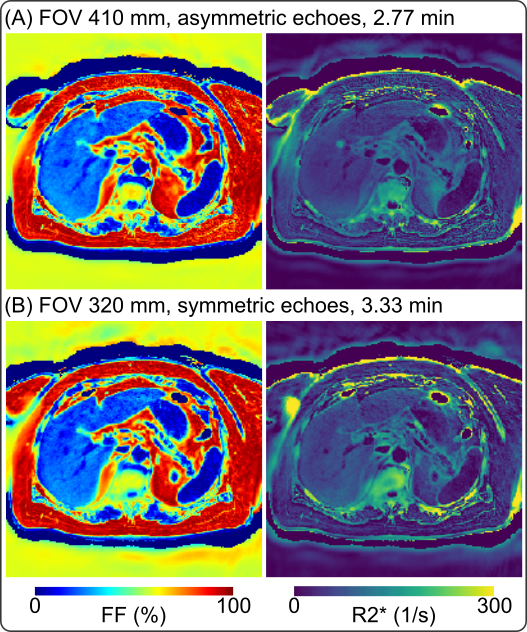
\includegraphics[width=0.6\textwidth]{../../figures/supp_tan1.png}
	\caption{Comparison between the protocols using 
		(A) asymmetric echoes with FOV $410$~mm and $2.77$~minutes scan time and 
		(B) symmetric echoes with FOV $320$~mm and $3.33$~minutes scan time.}
	\label{SUPPFIG:SYMM}
\end{figure}


	\item \textit{The description of the model based reconstruction in Eq. [5] needs to be expanded including the temporal dimension, the main unknowns and mathematical expressions for the E1 and E2 operators. The authors should also add to the formulation the Sobolev-norm weighting used for the field-map estimation. A separate formula should be included for the cost function minimized when only a L2 regularization is used, as showed later in the results section.}

\hspace{1em} Done.

	\item \textit{The authors compared three different methods: a breath-hold scan, a free-breathing scan reconstructed with only L2 regularization and a free-breathing scan reconstructed with the proposed method. Can the authors include a comparison to another free-breathing scan reconstruction technique exploiting the temporal variation like in the work in DOI: 10.1002/mrm.28280? Can the authors comment and show results on how their method compares to the previous work by Schneider et al?}

\hspace{1em} The work by Schneider et al.~employed spatial TV regularization 
on the water, fat, and $R_2^*$ maps, whereas $B_0$ field inhomogeneity and 
coil sensitivity maps were pre-calibrated. A comparison has been provided in Figure 5.

	\item \textit{The present work does not include important literature on the topic. Beyond the work by Schneider et al, there has been a significant amount of work aiming to perform free breathing liver PDFF and R2* mapping in DOI 10.1002/mrm.26693, DOI: 10.1002/mrm.28052 and many others. Please discuss the present work in the context of all previous works on the topic.}

\hspace{1em} Thank you for the suggestion. The above-mentioned literature have been cited.

\hspace{1em} 

\end{enumerate}

\noindent \textit{Minor Comments:}

\begin{enumerate}[resume]

	\item \textit{Abstract: I would label the cartesian scan as “reference” instead of “standard”.}

\hspace{1em} Done.

	\item \textit{Abstract: I would remove the phrase about replacing liver biopsy, as this is not really the focus of the present conclusions.}

\hspace{1em} Done.

	\item \textit{Introduction: On the 3rd paragraph the authors mix up two totally different concepts: a) B0 fluctuations induced by respiratory motion (resulting in a temporarily varying B0 map) and b) the fact that the field-map term is the non-linear term in the water-fat separation problem. Please rewrite this part highlighting the above two distinct technical challenges.}
	
\hspace{1em} Done.

	\item \textit{Introduction: More references should be added regarding techniques that enforce spatial smoothness to solve the field-map problem in water-fat imaging. This is a very well-studied topic.}

\hspace{1em} More references have been added.

	\item \textit{Introduction: “This work enables high-resolution free-breathing volumetric liver quantitative mapping with reduced scan time”. Where was it shown that the scan time was reduced?}

\hspace{1em} Please refer to Figure 10.

	\item \textit{Figure 6 could be enhanced by showing B0 maps at the 4 different bins to better highlight the reason for the R2* map overestimation at the upper liver region.}
	
\hspace{1em} Done.

\end{enumerate}

\vfill
\pagebreak

% ========================================
%     Reviewer 2
% ========================================

\noindent \underline{\textbf{Reviewer 2}}

\noindent \textit{Major Comments}

\begin{enumerate}
	\item \textit{For the phantom study, the Cartesian reference maps should be shown. If it was not acquired, the phantom experiment should be re-run to add it.}

\hspace{1em} For the phantom study, we encountered some difficulty using the reference Cartesian scan. Therefore, we used MRS instead.

	\item \textit{The phantom analysis currently ignores the ground truth fat fraction values, which are known by design. According to table I, tubes should be at 0\%, 10\%, 20\%, and 100\%. However, they are instead at 0\%, 13-14\%, 23-24\%, and not shown for both radial and MRS in Fig. 4. Why is fat being overestimated by both methods? MRS was not performed in the 100\% tube, but what was the radial value?}

\hspace{1em} The fat fraction values are "overestimated" due to the preparation of the phantom. We noticed steams coming from the water solution, which was heated at the hotplate at \SI{300}{\celsius} to create phantom emulsion. Therefore, the loss of water solution in the emulsion step resulted in "overestimation" of the fat fraction values.

	\item \textit{The radial R2* maps are quite blurry near the anterior-posterior midline in all patients (but not the volunteer), obscuring blood vessels that are visible in the Cartesian scan. This presumably causes some partial voluming issues for liver tissue quantification, and contradicts the subjective claim that the R2* maps are "sharp". Please discuss this observation, as well as any potential sources (e.g. poor coil sensitivity penetration deep in the body?).}

\hspace{1em} Thank you for the suggestion. We have added this into discussion.

	\item \textit{When discussing differences in R2* between breath-held Cartesian and the proposed method, the manuscript seems to give the benefit of the doubt to the proposed method (the Cartesian scan is described as "overestimated" or "underestimated"), even though the Cartesian breath-held scan is the (presumably regulatory-approved product) reference sequence.}

\hspace{1em} We acknowledge that the Cartesian breath-hold scan is the reference sequence. 
However, we observed in this study that in cases of incomplete breath hold, 
the reference sequence suffers from underestimated $R_2^*$, or in other words motion artifacts, 
as shown in Figures 5, 9 and 10.

	\item \textit{There is a parallelogram shape to the Bland-Altman FF plot in Fig. 7. This usually indicates some clipping in values for one or both methods. With magnitude discrimination, this could make sense on the bottom end of the FF range (water is more prevalent in this tissue), but these values are not near the high end of the FF range and should not be clipping there. There is also a potential negative slope to the differences, which may indicate that one method measured reduced population variablity. Both of these questions would be aided by the addition of scatter plots to Fig. 7, and the second question would be aided by the addition of a table with population descriptive statistics of FF and R2* over the subjects.}

\hspace{1em} Thank you for the suggestion. 
Scatter plots have been added to Figure 7. In addition, Table IV and V have been added.

	\item \textit{"As shown in figs.~10 and 11, retrospective undersampling increases noise in the reconstructed maps (larger standard deviation), but the quantitative accuracy agrees well with the reconstruction on 2:47 min scan (average values are similar)." Figs.~10 and 11 show the images and some scatter plots with error bars, but they do not directly show those findings. Those claims would require hypothesis testing to compare standard deviations between scan times and average values between scan times, respectively.}

\hspace{1em} Thank you for the suggestion. 
The standard deviations and average values have been added to Tables VI and V.

	\item \textit{What is the impact of the authors' choice to impose the LLR constraint on parameter maps rather than echo dimension? It's an intriguing option that is only available to model-based methods, but hasn't been compared or discussed.}

\hspace{1em} Thank you for the suggestion. We added this into Discussion.

	\item \textit{Although the approach here to free-breathing volumetric liver quantitative mapping of R2* and B0 has differences from other approaches, the manuscript is not always clear on what those exact differences are, nor what additional capabilities might be enabled by those differences. \\
	Capabilities: The introduction says this work "enables high-resolution free-breathing volumetric liver quantitative mapping with reduced scan time", but which part of that is being enabled? Free-breathing volumetric liver quantitative mapping of R2* and B0 exists:
	Zhong et al. (doi.org/10.1002/jmri.27205) and followups
	Schneider et al. (Manuscript reference 26)
	Wang et al. (doi.org/10.1002/mrm.28970)
	Starekova et al. (doi.org/10.1007/s00330-022-08682-x)
	Is the difference here the resolution and scan time?\\
	Methodology: "to the best of our knowledge, there has been no previous work on joint estimation of all parameter maps in free-breathing multi-echo chemical shift imaging, i.e. water, fat, $R_2^*$, B0 field inhomogeneity maps, and coil sensitivity maps". The above references seemingly estimate these maps from one free-breathing scan, although not all reports are clear on their source of sensitivity maps. Is the main difference the simultaneous alternating estimation? If so, can the authors show or discuss the advantages and disadvantages of this difference?}

\hspace{1em} Our approach jointly estimates all parameter maps (water, fat, $R_2^*$, and $B_0$) 
and coil sensitivity maps directly from the acquired $k$-space data. 
This reconstruction approach is known as model-based reconstruction, which, in general, 
solves a regularized nonlinear inverse problem directly from the measured $k$-space data. 
This work developed an integrated algorithm based on 
the iteratively regularized Gauss-Newton method (IRGNM) and 
the alternating direction method of multipliers (ADMM). 

\hspace{1em} In contrast, the other approaches (Zhong et al., Wang et al., and Starekova et al.) 
solved the quantification problem in two steps: 
(1) reconstruction of all echo images, and (2) image-space parameter fitting. 

\hspace{1em} Another relevant work based on model-based reconstruction is from Schneider et al., 
which employed spatial total variation regularization on parameter maps. 
Moreover, Schneider et al.~pre-calibrated $B_0$ and coil sensitivity maps, 
which were then kept constant during model-based reconstruction.

\end{enumerate}

\noindent \textit{Minor Comments}

\begin{enumerate}[resume]
	\item \textit{The introduction should discuss/review previous free-breathing approaches, and place this method's approach to free-breathing (self-gating and temporal TV) in that context.}

\hspace{1em} Done.

	\item \textit{The L and TV\_t operators in Eq. 5 are not directly defined in the text.}

\hspace{1em} Done.

	\item \textit{Where is the Sobolev-norm weighting in Eq.~5?}

\hspace{1em} Thank you. It has been added.

	\item \textit{Exactly which maps do E1 and E2 extract?}

\hspace{1em} Thank you. The operator has been explained.

	\item \textit{Please provide more detail on the reference Cartesian method. is the Siemens qDIXON package? Is there a citation? What fitting model does it use?}

\hspace{1em} Yes, it is the Siemens qDixon package. A citation has been added. 
Its fitting model is the same as in Equation (3).

	\item \textit{For the reference method, was the breath-hold after expiration or inspiration? For figures that show only one respiratory phase, which was it: end expiration or end inspiration? Comparisons should choose the same phase as the breath-hold to minimize respiratory mismatch and ensuing differences in R2*.}

\hspace{1em} The breath-hold was performed after expiration.

	\item \textit{Was shimming done after expiration, inspiration, or during free breathing? This may provide further context to any differences in R2* between the breath-held and free-breathing scan.}

\hspace{1em} Shimming was done during free breathing.

	\item \textit{Table III is referenced as to the obesity diagnosis of one of the patients, but the diagnosis is not actually in the table. Can the authors add a column either listing the diagnoses or the criteria (e.g., BMI) for those diagnoses?}

\hspace{1em} Done.

	\item \textit{The subscript to lambda is serving double-duty here. Sometimes it refers to the three different parameters in Eq. 5, but sometimes it refers to the Newton iteration number. Please clarify.}

\hspace{1em} Thank you for this comment. We have clarified its meaning in the manuscript.

	\item \textit{FF is being calculated as $1 - |\text{W}|/|\text{W}+\text{F}|$, but Page 2 says that both W and F are allowed to be complex. Could phase mismatch occur, causing underestimation of FF?  Is this what the authors mean in patient \#6, when they say the lower FF for the proposed method "might be due to the use of magnitude discrimination"? Magnitude discrimination was a choice by the authors, so don't you have the data to confirm this rather than speculating?}

\hspace{1em} Thank you for the suggestion. We observed that the FF values of 
Patient \#6 is lower than the reference Cartesian scan, 
as shown in Figure 7 and Table IV in the manuscript.

\hspace{1em} As suggested, we compared three FF calculation methods: 
$|\mathrm{F}|/(|\mathrm{W} + \mathrm{F}|)$, 
$1 - |\mathrm{W}|/(|\mathrm{W} + \mathrm{F}|)$, and 
$1 - |\mathrm{W}|/(|\mathrm{W}| + |\mathrm{F}|)$. 
The latter two methods use magnitude discrimination.
\cref{SUPPFIG:FATFRAC} shows the corresponding FF maps from Patient \#6 and \#9, respectively.
Mean and standard deviation of three region of interests from the calculated FF maps are listed 
in \cref{SUPPTAB:FATFRAC}. 
In general, the use of magnitude discrimination yields slightly lower FF values. 
On the other hand, since both W and F are allowed to be complex, 
we use the third method for the calculation of FF, 
i.e.~$\mathrm{FF} = 1 - |\mathrm{W}| / (|\mathrm{W}| + |\mathrm{F}|)$.

\begin{figure}[h!]
	\centering
	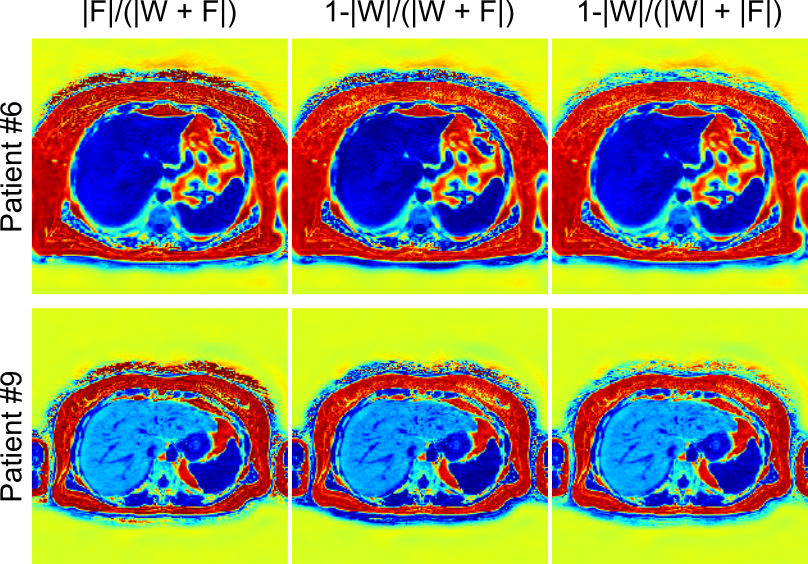
\includegraphics[width=0.6\textwidth]{../../figures/supp_tan2.png}
	\caption{Comparison among three fat fraction calculation methods: 
		(left) $|\mathrm{F}| / (|\mathrm{W} + \mathrm{F}|)$, 
		(middle) $1 - |\mathrm{W}| / (|\mathrm{W} + \mathrm{F}|)$, and 
		(right) $1- |\mathrm{W}| / (|\mathrm{W}| + |\mathrm{F}|)$.}
	\label{SUPPFIG:FATFRAC}
\end{figure}

\begin{table}[h!]
	\caption{Mean and standard deviation of the fat fraction maps from \cref{SUPPFIG:FATFRAC}.}
	\begin{tabular}{m{0.14\textwidth} m{0.22\textwidth} m{0.17\textwidth} m{0.17\textwidth} m{0.17\textwidth}}
		\toprule
		& & ROI \#1 & ROI \#2 & ROI \#3 \\
		\hline
		\multirow{3}{*}{Patient \#6} & $|\mathrm{F}|/(|\mathrm{W} + \mathrm{F}|)$ & $4.85 \pm 1.83$ & $7.95 \pm 1.22$ & $10.07 \pm 1.32$ \\
		& $1 - |\mathrm{W}|/(|\mathrm{W} + \mathrm{F}|)$ & $3.41 \pm 2.02$ & $4.90 \pm 1.41$ & $8.09 \pm 1.44$ \\
		& $1 - |\mathrm{W}|/(|\mathrm{W}| + |\mathrm{F}|)$ & $4.77 \pm 1.75$ & $7.71 \pm 1.16$ & $9.87 \pm 1.28$ \\
		\midrule
		\multirow{3}{*}{Patient \#9} & $|\mathrm{F}|/(|\mathrm{W} + \mathrm{F}|)$ & $29.63 \pm 2.82$ & $29.69 \pm 2.27$ & $29.97 \pm 1.24$ \\
		& $1 - |\mathrm{W}|/(|\mathrm{W} + \mathrm{F}|)$ & $28.70 \pm 2.93$ & $28.45 \pm 2.50$ & $29.14 \pm 1.32$ \\
		& $1 - |\mathrm{W}|/(|\mathrm{W}| + |\mathrm{F}|)$ & $29.36 \pm 2.80$ & $29.33 \pm 2.29$ & $29.72 \pm 1.24$ \\
		\bottomrule
	\end{tabular}
	\label{SUPPTAB:FATFRAC}
\end{table}

	\item \textit{Why is the fat so much noiser for radial imaging in FF maps? Is this because of the magnitude discrimination again?}

\hspace{1em} As shown in the answer to (18), 
the use of magnitude discrimination does not increase standard deviation. 
In comparison to the reference Cartesian scan with the in-plane pixel size \SI{2.56}{\mm\square}, 
the proposed radial scan supplies smaller pixel size \SI{1.60}{\mm\square}. 
The use of smaller pixel size also result in intrinsic SNR penalty. 
Note that reducing the pixel size in the reference Cartesian protocol to \SI{1.60}{\mm\square} 
is not feasible as it will require longer breath hold.

	\item \textit{Colormaps rather than grayscale maps would be very helpful for viewing results.}

\hspace{1em} Done.

	\item \textit{"Both Cartesian and radial scans provide comparable FF maps." Comparable in what sense?}

\hspace{1em} As suggested above, we have included Bland-Altman plots, scatter plots, as well as tables with mean and standard deviation values between Cartesian and radial scans for the comparison of FF values.

	\item \textit{The discussion says that unaligned kz undersampling would be more computationally challenging, but also offers kz undersampling as a way to accelerate reconstruction time. Please resolve this apparent contradiction.}

\hspace{1em} Done.

	\item \textit{The discussion also says that with unaligned kz undersampling, "expensive 3D image reconstruction would be required". This is 3D reconstruction already, not slice-by-slice, right? Or is the smoothness on B0 and coil maps only being imposed in the x-y plane? Please clarify.}

\hspace{1em} Thank you for the question. For the stack-of-stars acquisition, 
3D k-space data is firstly to slices via 1D FFT along the $k_z$ dimension. 
Afterwards, reconstruction can be done for every slice. 
Therefore, the smoothness on $B_0$ and coil maps is imposed in the x-y plane.

	\item \textit{Pilot tone binning is mentioned but not cited.}

\hspace{1em} Done.

	\item \textit{There are several typos and minor language issues that would benefit from another round of proofreading.}

\hspace{1em} Thank you for the suggestion. We have conducted language grammar checks and proofreading.

\end{enumerate}

\vfill
\pagebreak

% ========================================
%     Reviewer 3
% ========================================

\noindent \underline{\textbf{Reviewer 3}}

\noindent \textit{Major Comments:}

\begin{enumerate}
	\item \textit{I am worried about the lack of technical novelty of the work. In the second Section ("Theory"), only the design of the sequence has some novelty. The authors should emphasize the novelty of the whole work much more in the Introduction part and Theory part. Otherwise, I cannot support the publication of the manuscript in its current form with enough enthusiasm.}

\hspace{1em} Thank you for the suggestion. Beside the sequence design, 
another contribution of this work is the model-based reconstruction, 
which jointly estimates all parameter maps (water, fat, $R_2^*$ and $B_0$) and 
coil sensitivity maps directly from the measured $k$-space data. 
In addition, we have also emphasized our work in Introduction and Theory.

	\item \textit{The notations in the manuscript are not well-explained. At least all the used notations should be explained. The authors should pay much more attention to the notations used in the manuscript to make all the equations clear. For example, I am confused by the second part of eq. (4). I think more explanations are needed here for eq. (4). Another example is that in eq. (5), what is $\mathcal{L}$? And the $E_1$ and $E_2$ operators are pretty abstract.}

\hspace{1em} We have enhanced explanations of notations an equations in the manuscript.

	\item \textit{For the model-based reconstruction, the initialization seems to be problematic. As the authors mentioned in the manuscript, the W, F and $f_{B_0}$ need to be initialized using another model-based method. This significantly affects the effectiveness of the whole reconstruction algorithm. If an algorithm has to use some very good initial guess from somewhere else, then it's hard to appreciate the current used method. Is it possible to come up with a way so that the reconstruction will work for a more general initialization in this work as this is urgently needed for this work (not future work)?}

\hspace{1em} Only $f_{B_0}$ is initialized from the 3-echo model-based reconstruction. 
We have corrected this in the manuscript. 
Note that Schneider et al.~pre-calibrated the $B_0$ map instead (This calibrated $B_0$ map is kept constant during model-based reconstruction). 
Our work already allowed for the joint update of $B_0$ maps for every respiratory bins.


	\item \textit{From the results shown in the manuscript, seems that the fat fraction and $R_2^*$ estimated from the proposed scheme is consistently higher than the estimation from the breath-hold cartesian data. Is this excepted? I think a phantom study is needed to investigate this problem so that we may know which estimation is more accurate.}

\hspace{1em} We would argue against that the fat fraction and $R_2^*$ values 
estimated from the proposed scheme are consistently higher than 
the reference breath-hold Cartesian scan. First, beside the Bland-Altman plots, 
we have also included scatter plots in Figure 7 in the manuscript. 
These plots show good match between the proposed radial and the reference Cartesian methods. 
Second, Tables IV and V in the manuscript summarize the mean and standard deviation values 
of all ROIs and all patients. 

	\item \textit{One of the goals of this work is to estimated the $B_0$ filed maps and coil sensitivity maps. But there is no result on the coil sensitivity maps is shown in the manuscript, and there is no $B_0$ filed map result for in vivo datasets. Since the authors proposed to estimate the $B_0$ filed maps and coil sensitivity maps, the results of $B_0$ filed maps and coil sensitivity maps should be shown in the manuscript. I am curious to see the coil sensitivity map estimation comparing to other coil sensitivity map estimation methods (e.g. ESPIRiT or J-SENSE coil sensitivity map estimation).}

\hspace{1em} Thank you for the suggestion. $B_0$ field maps have been added to Figure 6 in the manuscript. In addition, \cref{SUPPFIG:SENS} shows the coil sensitivity maps estimated 
from the proposed model-based reconstruction and ESPIRiT 
\footnote{Uecker M, et al. ESPIRiT -- An eigenvalue approach to autocalibrating parallel MRI: Where SENSE meets GRAPPA. \textit{Magn Reson Med} 2014;71:990--1001}, respectively.

\begin{figure}[t]
	\centering
	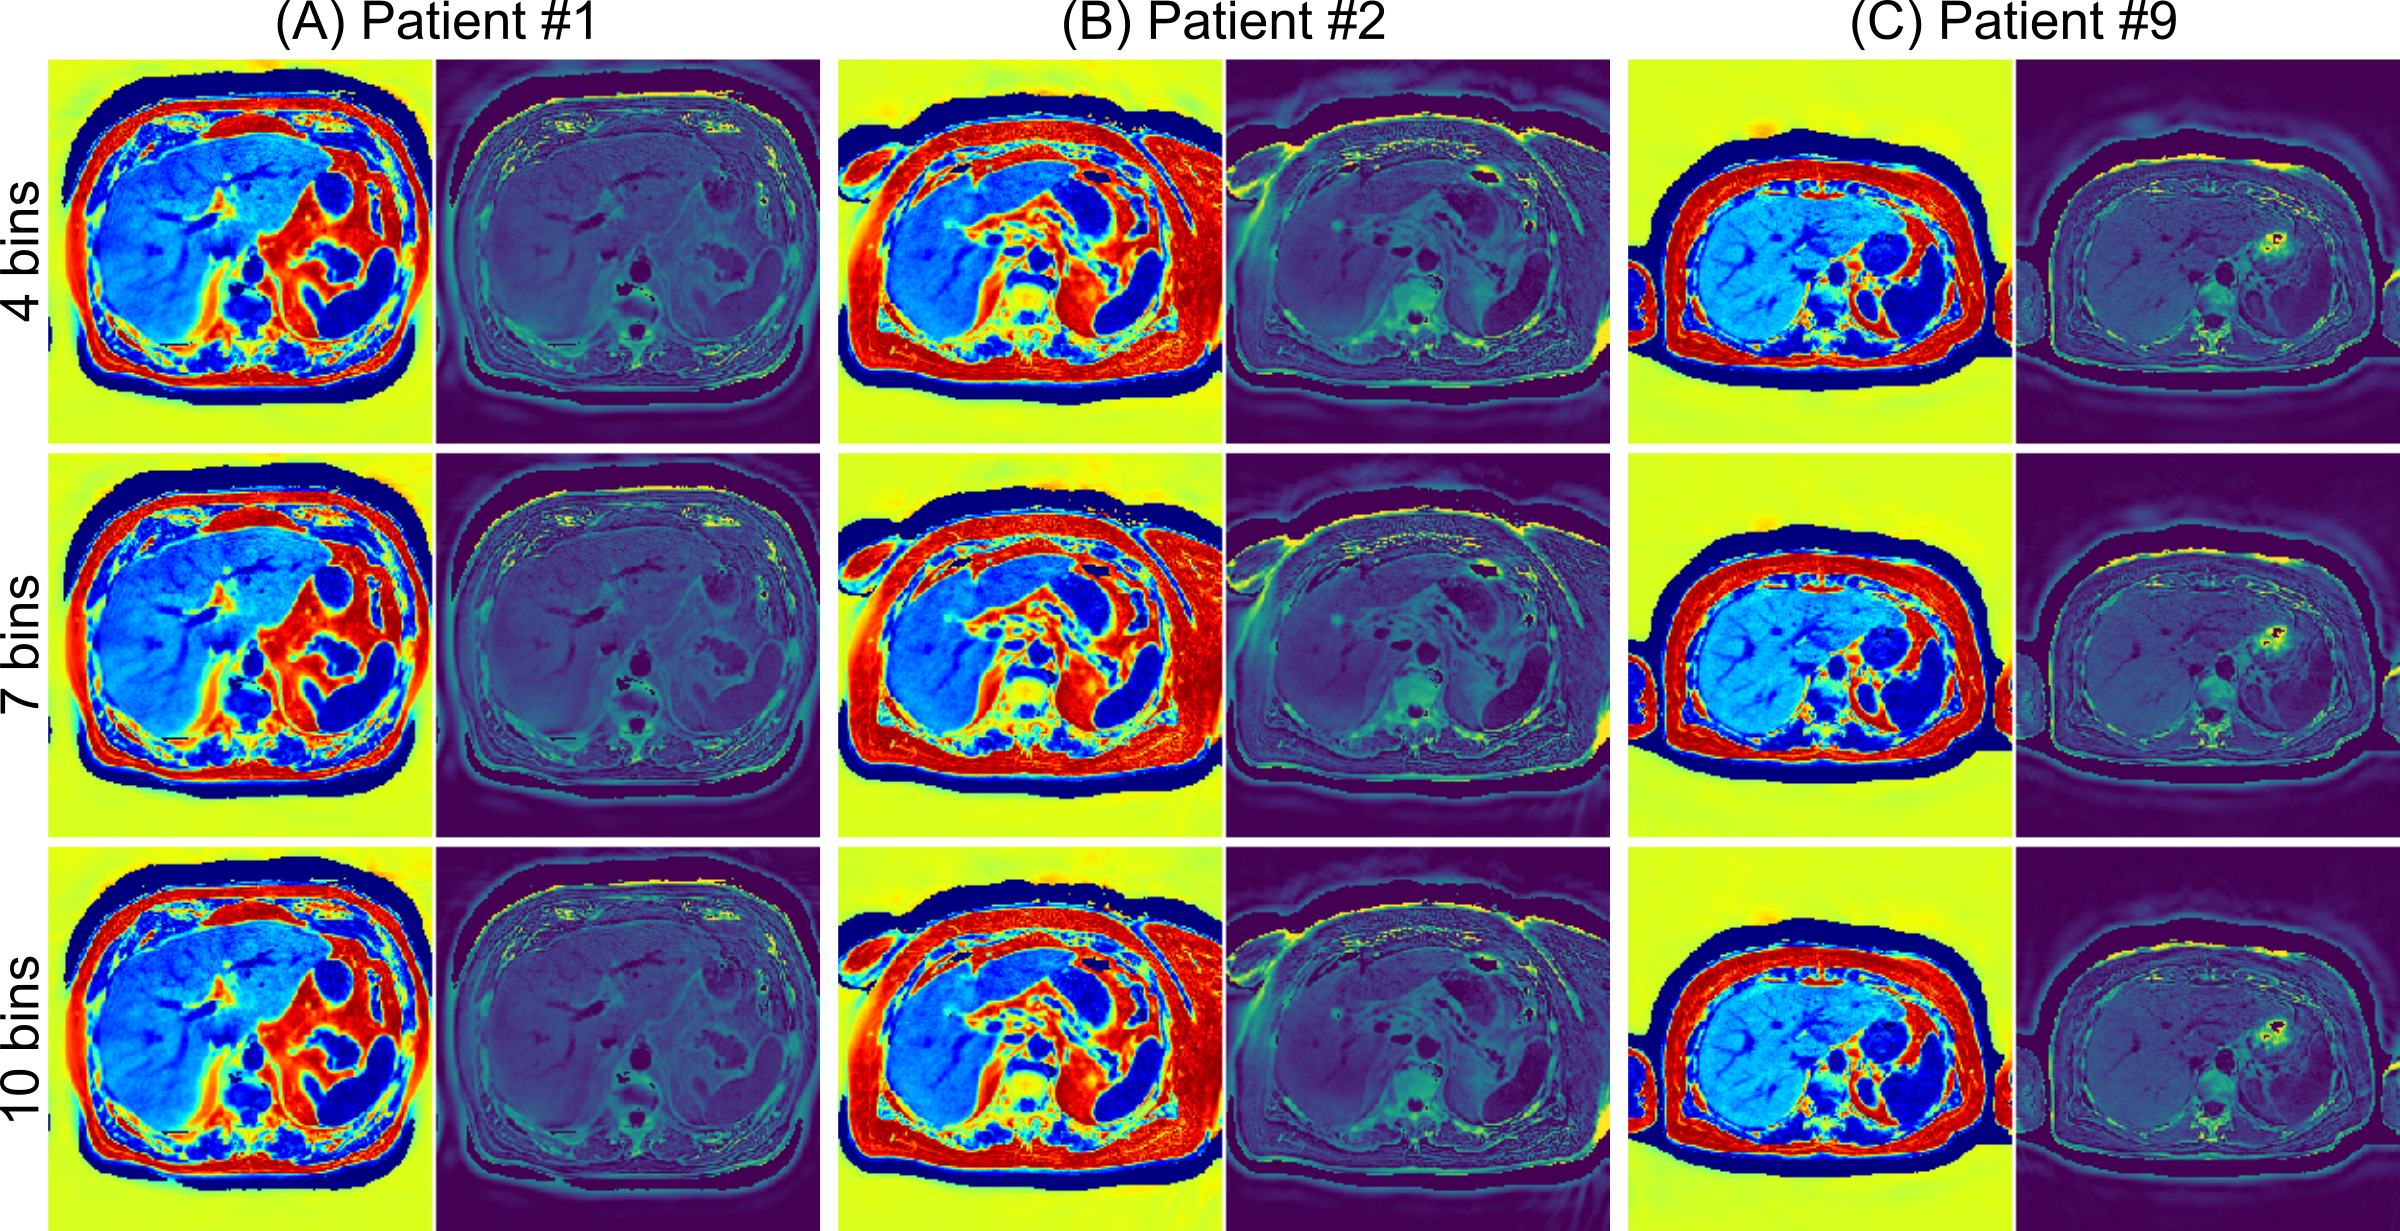
\includegraphics[width=\textwidth]{../../figures/supp_tan3.png}
	\caption{Comparison of coil sensitivity maps in (A) Patient \#1 and (B) Patient \#2 
		from the proposed model-based reconstruction and ESPIRiT, respectively.}
	\label{SUPPFIG:SENS}
\end{figure}



\end{enumerate}

\noindent \textit{Minor Comments:}

\begin{enumerate}[resume]

	\item \textit{For the phantom study, why don't the authors also do the Cartesian scan and compared the results obtained from the Cartesian scan with the results using the proposed sequence? If so, we can have a better understanding about the effectiveness of the proposed scheme.}

\hspace{1em} For the phantom study, we encountered some difficulty using the reference Cartesian scan. 
Therefore, we used MRS instead.

	\item \textit{In Fig.5, which shows the results from Patient \#1, I can clearly see that the there is heavy blurring, which affects the estimation (e.g., the estimation of the liver region in the left bottom of the image are strongly affected by the blurring). I am not sure the blurring comes from the too strong regularization or it comes from the less number of bins (only 4 bins are used). But definitely this issue needs to be further investigated.}

\hspace{1em} As shown in Table III in the manuscript, Patient \#1 has relatively large body size, 
which may cause poor coil sensitivity penetration in the body, as mentioned by Reviewer 2. 
On the other hand, to investigate whether the use of 4 respiratory bins is insufficient 
to resolve motion, we display in \cref{SUPPFIG:BINS} the reconstruction results 
from Patient \#1, \#2 and \#9 with 4, 7, and 10 bins, respectively.
Admittedly, the result from Patient \#1 is more blurry than other patients. 
Increasing the number of respiratory bins does not seem to reduce blurring. 


\begin{figure}[t]
	\centering
	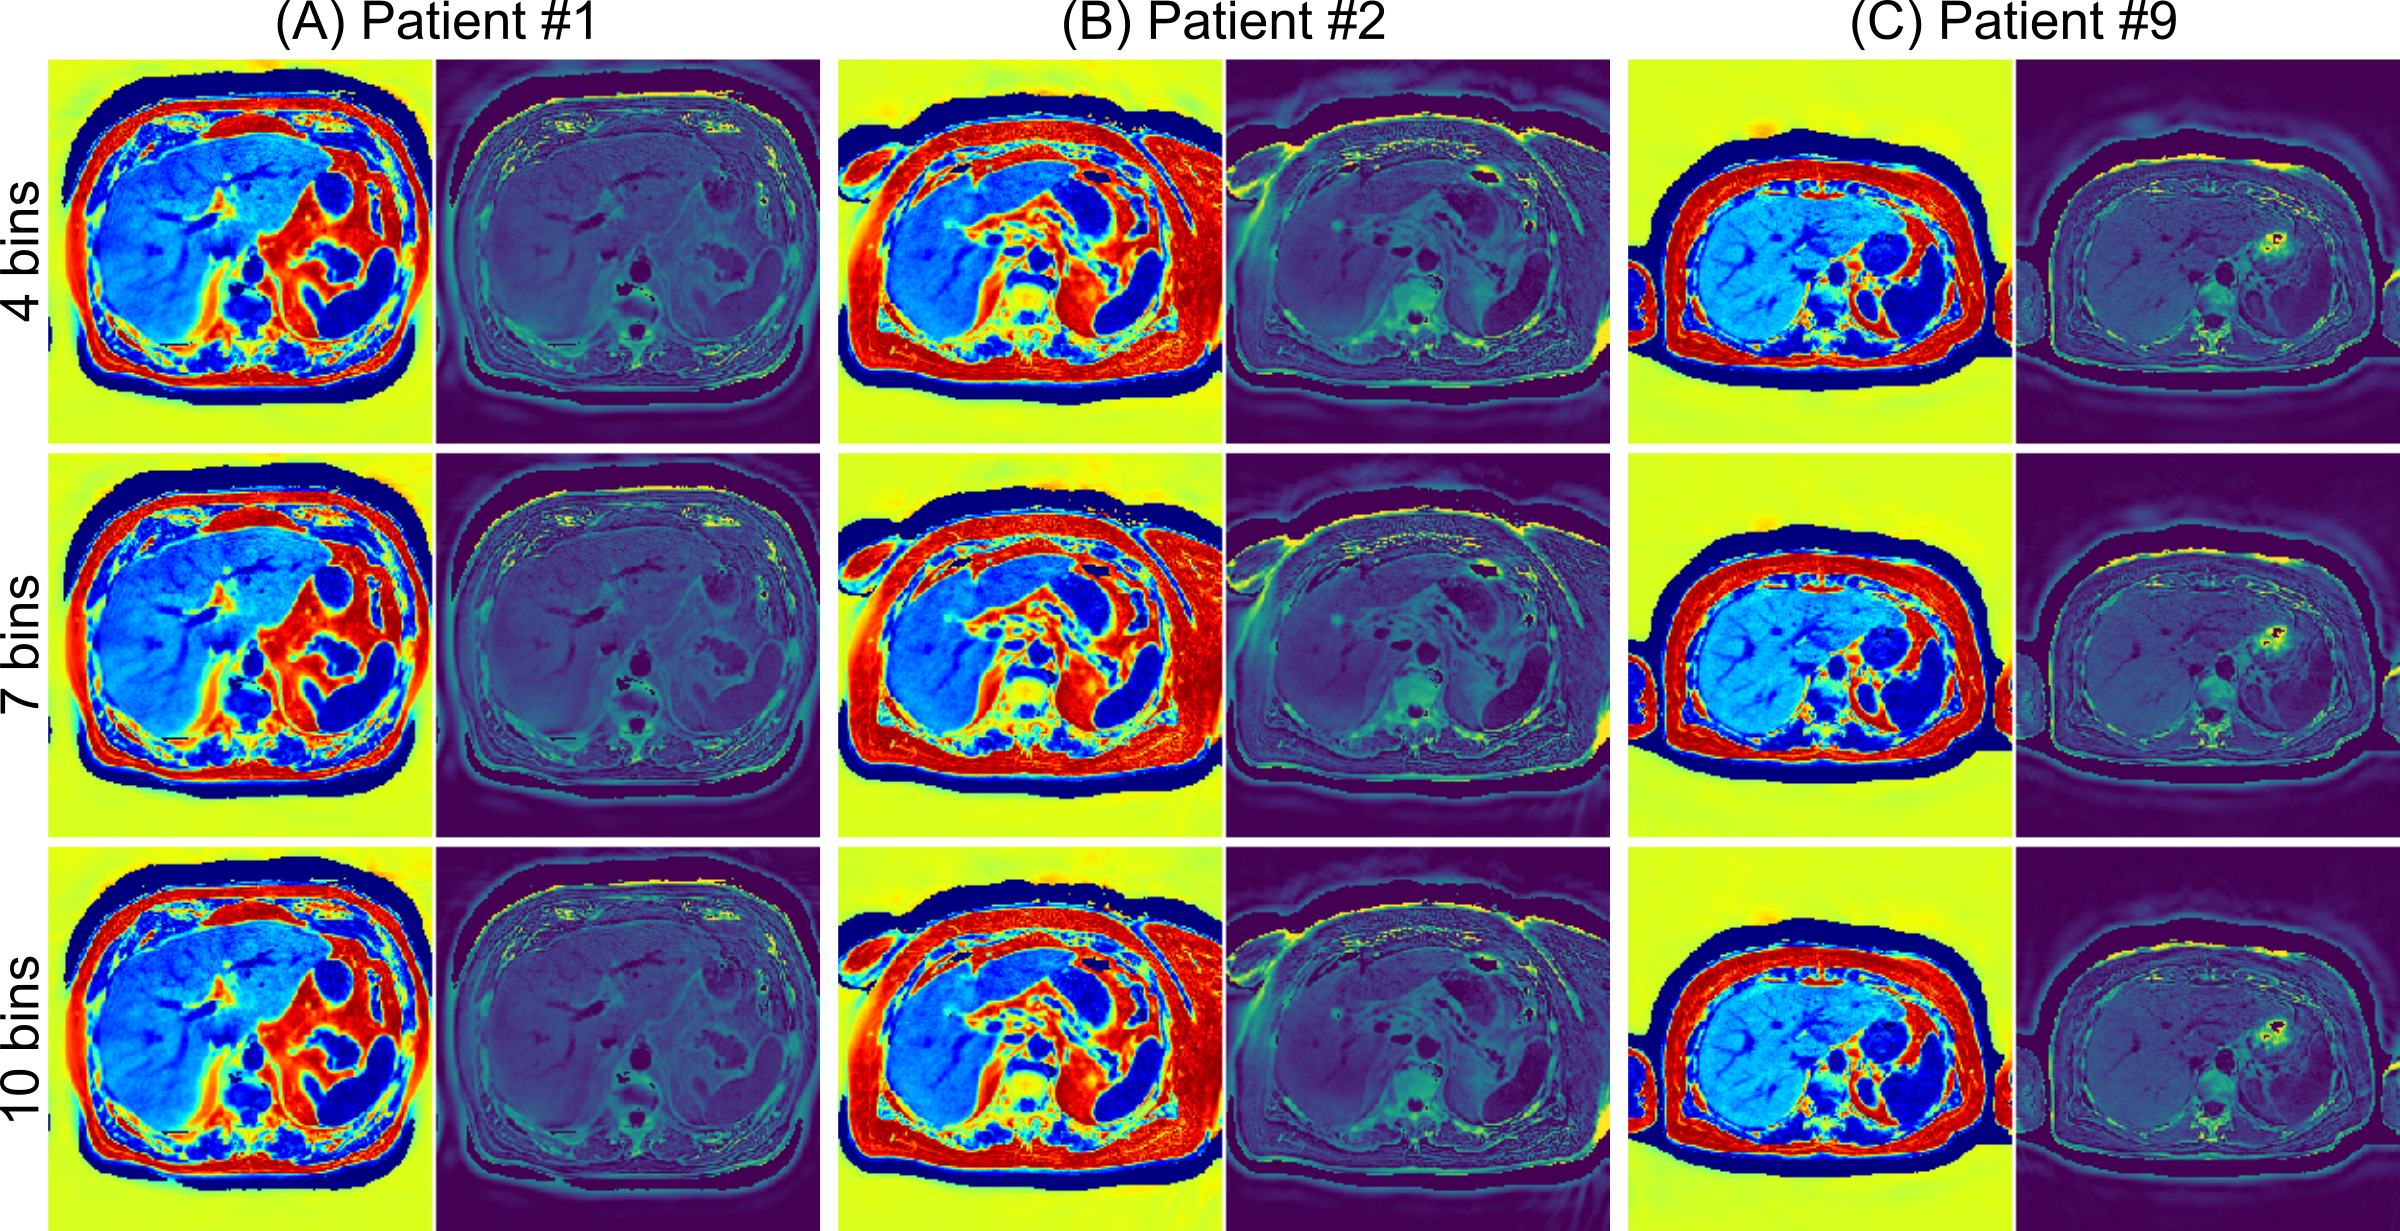
\includegraphics[width=\textwidth]{../../figures/supp_tan4.png}
	\caption{Investigation on the number of respiratory bins used for model-based reconstruction.
	Displayed images are the FF and $R_2^*$ maps from (A) Patient \#1, (B) Patient \#2, and (C) Patient \#9, respectively.}
	\label{SUPPFIG:BINS}
\end{figure}

	\item \textit{In Section III. B, it says "Further, we investigated the effectiveness of the proposed motion-resolved ......, which corresponds to half of the total scan time." I am not sure what does this mean. Can you explain more?}

\hspace{1em} This means that we retrospectively cut out the second half of the acquired data. 
With the reduced data, we then perform image reconstruction.

	\item \textit{The reconstruction time takes about 4 hours, even with only 4 bins and using the Tesla V100 GPU. I think to make the work stronger and gain more practical value, it is worthwhile for considering more on how to speed up the reconstruction.}

\hspace{1em} Thank you for the suggestion. We have discussed this issue in Discussion.

\end{enumerate}

\end{document}
